\chapter{Complete Link Budget Analysis}
\label{ch:link-budget}

\begin{nontechnical}
\textbf{Link budget is like a financial budget for radio power}---you start with transmit power, subtract losses, add gains, and see if there's enough ``money'' (signal) left at the receiver!

\textbf{The fundamental question:} ``If I transmit from HERE to THERE, will the receiver get enough signal?''

\textbf{The accounting:}

\textbf{START (Transmit power):}
\begin{itemize}
\item WiFi router: 100~mW (20~dBm)
\item Cell tower: 20~W (43~dBm)
\item Satellite: 100~W (50~dBm)
\end{itemize}

\textbf{GAINS (things that help):}
\begin{itemize}
\item \textbf{Transmit antenna gain:} Directional antenna focuses power
  \begin{itemize}
  \item WiFi router: $+2$~dB
  \item Satellite dish: $+40$~dB (very focused!)
  \end{itemize}
\item \textbf{Receive antenna gain:} Bigger antenna collects more
  \begin{itemize}
  \item Phone: $0$~dB (tiny antenna)
  \item Satellite dish: $+35$~dB
  \end{itemize}
\end{itemize}

\textbf{LOSSES (things that hurt):}
\begin{itemize}
\item \textbf{Free-space path loss:} Signal spreads with distance
  \begin{itemize}
  \item WiFi (50~m): $-74$~dB
  \item Cell tower (1~km): $-100$~dB
  \item Satellite (36,000~km): $-206$~dB!
  \end{itemize}
\item \textbf{Obstacles:} Walls, trees, rain
  \begin{itemize}
  \item One wall: $-5$~dB
  \item Heavy rain: $-10$~dB
  \end{itemize}
\item \textbf{Cable losses:} Connectors, cables ($-1$ to $-3$~dB)
\end{itemize}

\textbf{END (Received power):} Must be stronger than noise floor! Typical requirement: Signal $>$ Noise $+ 10$ to $20$~dB.

\textbf{Real example---WiFi link:} Transmit 20~dBm $+$ antenna 2~dB $= $ 22~dBm EIRP. Subtract free-space loss 74~dB and wall loss 10~dB $= -62$~dBm received. Noise floor $-90$~dBm gives SNR $= 28$~dB. Link works!

\textbf{Fun fact:} Voyager~1 spacecraft (over 13 billion miles away) transmits at 23~W. By the time it reaches Earth, the signal is $10^{-16}$~watts! Only massive 70-meter dishes with careful link budgets can hear it.
\end{nontechnical}

\section{Overview}

\textbf{Link budget} is a comprehensive accounting of \textbf{all gains and losses} from transmitter to receiver, determining whether a communication link will function reliably under specified conditions.

\begin{keyconcept}
Link budget analysis answers the critical question: \textbf{``Will the receiver obtain sufficient signal power to achieve the required data rate and bit error rate?''}
\end{keyconcept}

The fundamental link budget equation expresses received power in logarithmic units (dBm or dBW):
\begin{equation}
P_r = P_t + G_t - L_{\text{total}} + G_r
\label{eq:link-budget-basic}
\end{equation}
where:
\begin{itemize}
\item $P_r$ = received signal power (dBm)
\item $P_t$ = transmit power (dBm)
\item $G_t$ = transmit antenna gain (dBi)
\item $L_{\text{total}}$ = total path loss (dB)
\item $G_r$ = receive antenna gain (dBi)
\end{itemize}

\textbf{Link closure criterion:}
\begin{equation}
P_r > P_{\text{min}}
\label{eq:link-closure}
\end{equation}
where $P_{\text{min}}$ is the receiver sensitivity (minimum detectable signal).

\textbf{Link margin:}
\begin{equation}
M = P_r - P_{\text{min}} \quad \text{(dB)}
\label{eq:link-margin}
\end{equation}

The margin $M$ provides a safety buffer against fading, interference, and implementation losses. Positive margin is required for link closure; typical design targets range from 10 to 30~dB depending on the application.

\section{Link Budget System Overview}

A complete link budget encompasses transmitter, propagation path, and receiver subsystems. Figure~\ref{fig:link-budget-system} illustrates the end-to-end signal flow and associated gains and losses.

\begin{center}
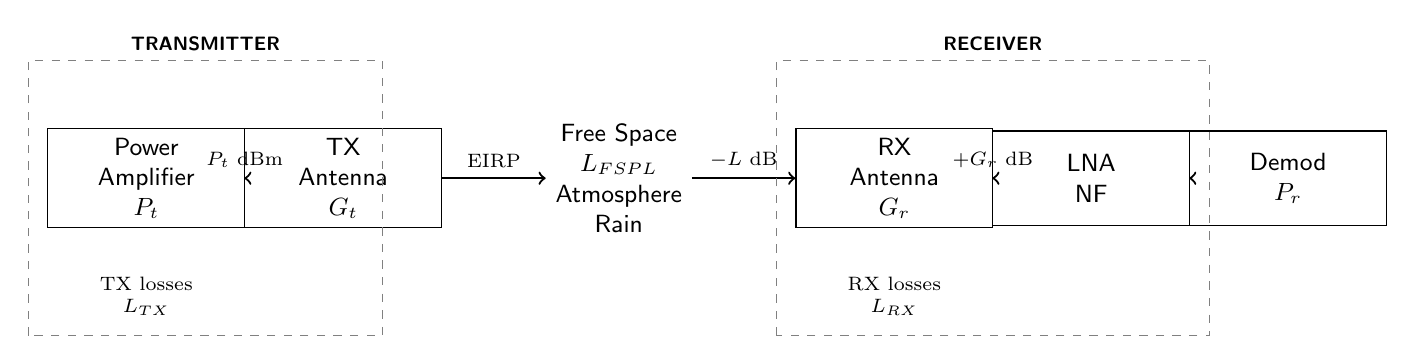
\begin{tikzpicture}[
  block/.style={rectangle, draw, minimum width=2.5cm, minimum height=1.2cm, font=\sffamily\small, align=center},
  gain/.style={isosceles triangle, draw, shape border rotate=0, minimum width=1cm, minimum height=1.2cm, font=\sffamily\scriptsize},
  node distance=1.8cm,
  font=\small
]
% Transmitter chain
\node[block] (pa) {Power\\Amplifier\\$P_t$};
\node[block, right of=pa, node distance=2.5cm] (txant) {TX\\Antenna\\$G_t$};

% Path
\node[right of=txant, node distance=3.5cm, align=center, font=\sffamily\small] (path) {Free Space\\$L_{\text{FSPL}}$\\Atmosphere\\Rain};

% Receiver chain
\node[block, right of=path, node distance=3.5cm] (rxant) {RX\\Antenna\\$G_r$};
\node[block, right of=rxant, node distance=2.5cm] (lna) {LNA\\NF};
\node[block, right of=lna, node distance=2.5cm] (demod) {Demod\\$P_r$};

% Signal flow
\draw[->,thick] (pa) -- node[above,font=\scriptsize] {$P_t$~dBm} (txant);
\draw[->,thick] (txant) -- node[above,font=\scriptsize] {EIRP} (path);
\draw[->,thick] (path) -- node[above,font=\scriptsize] {$-L$~dB} (rxant);
\draw[->,thick] (rxant) -- node[above,font=\scriptsize] {$+G_r$~dB} (lna);
\draw[->,thick] (lna) -- (demod);

% Loss/gain annotations
\node[below of=pa, node distance=1.5cm, font=\scriptsize, align=center] {TX losses\\$L_{\text{TX}}$};
\node[below of=rxant, node distance=1.5cm, font=\scriptsize, align=center] {RX losses\\$L_{\text{RX}}$};

% System boundaries
\draw[dashed, gray] (-1.5,-2) rectangle (3,1.5);
\node[above, font=\sffamily\scriptsize\bfseries] at (0.75,1.5) {TRANSMITTER};

\draw[dashed, gray] (8,-2) rectangle (13.5,1.5);
\node[above, font=\sffamily\scriptsize\bfseries] at (10.75,1.5) {RECEIVER};
\end{tikzpicture}
\end{center}

\section{Link Budget Components}\label{link-budget-components}

\subsection{Transmitter Side}

\subsubsection{Transmitted Power}

The transmitted power $P_t$ is the RF power delivered to the transmit antenna after accounting for all losses in the transmitter chain:
\begin{equation}
P_t = P_{\text{amp}} - L_{\text{TX}}
\label{eq:tx-power}
\end{equation}
where:
\begin{itemize}
\item $P_{\text{amp}}$ = power amplifier output power (dBm)
\item $L_{\text{TX}}$ = transmitter losses including cables, filters, circulators, and connectors (dB)
\end{itemize}

\begin{calloutbox}{Example: WiFi Router Transmit Power}
\textbf{Given:}
\begin{itemize}
\item PA output: $P_{\text{amp}} = 20$~dBm (100~mW)
\item Cable/connector loss: $L_{\text{TX}} = 0.5$~dB
\end{itemize}

\textbf{Solution:}
\begin{equation*}
P_t = 20 - 0.5 = 19.5\text{~dBm}
\end{equation*}
\end{calloutbox}

\subsubsection{Transmit Antenna Gain and EIRP}

The transmit antenna gain $G_t$ is measured relative to an isotropic radiator and expressed in dBi. The combination of transmit power and antenna gain yields the \textbf{Effective Isotropic Radiated Power (EIRP)}:
\begin{equation}
\text{EIRP} = P_t + G_t
\label{eq:eirp}
\end{equation}

\textbf{Example:} For $P_t = 19.5$~dBm and $G_t = 2$~dBi (omnidirectional WiFi antenna):
\begin{equation*}
\text{EIRP} = 19.5 + 2 = 21.5\text{~dBm}
\end{equation*}

\begin{warningbox}
\textbf{Regulatory compliance is mandatory.} Most jurisdictions limit EIRP to prevent interference. For example, FCC regulations limit EIRP to 36~dBm (4~W) for unlicensed 2.4~GHz WiFi operations. Exceeding these limits can result in legal penalties and harmful interference to other systems.
\end{warningbox}

\subsection{Propagation Path}

\subsubsection{Free-Space Path Loss}

Free-space path loss (FSPL) quantifies the attenuation of electromagnetic waves propagating through free space due to spherical wavefront expansion. The loss is derived from the Friis transmission equation:
\begin{equation}
L_{\text{FSPL}} = 20\log_{10}(d) + 20\log_{10}(f) + 20\log_{10}\left(\frac{4\pi}{c}\right)
\label{eq:fspl-full}
\end{equation}
where:
\begin{itemize}
\item $d$ = distance between transmitter and receiver (m)
\item $f$ = frequency (Hz)
\item $c = 3 \times 10^8$~m/s = speed of light
\end{itemize}

\textbf{Practical form} with distance in kilometers and frequency in MHz:
\begin{equation}
L_{\text{FSPL}} = 32.45 + 20\log_{10}(d_{\text{km}}) + 20\log_{10}(f_{\text{MHz}})
\label{eq:fspl-practical}
\end{equation}

\begin{calloutbox}{Example: WiFi Free-Space Path Loss}
\textbf{Given:}
\begin{itemize}
\item Frequency: $f = 2.4$~GHz $= 2400$~MHz
\item Distance: $d = 100$~m $= 0.1$~km
\end{itemize}

\textbf{Solution:}
\begin{align*}
L_{\text{FSPL}} &= 32.45 + 20\log_{10}(0.1) + 20\log_{10}(2400) \\
&= 32.45 - 20 + 67.6 \\
&= 80.0\text{~dB}
\end{align*}
\end{calloutbox}

\textbf{Cross-reference:} See Chapter~\ref{ch:fspl} for detailed derivation and frequency dependence analysis.

\subsubsection{Atmospheric Absorption}

Oxygen and water vapor molecules exhibit resonant absorption at specific frequencies, producing additional attenuation. This effect becomes significant above 10~GHz and must be accounted for in satellite and millimeter-wave links.

\textbf{Zenith attenuation at sea level:}

\begin{center}
\begin{tabular}{@{}lll@{}}
\toprule
Frequency & Attenuation (dB/km) & Notes \\
\midrule
$< 10$~GHz & $< 0.01$ & Negligible \\
22.2~GHz & 0.2 & H$_2$O resonance \\
60~GHz & 15 & O$_2$ resonance (peak) \\
120~GHz & 2 & Secondary O$_2$ line \\
183~GHz & 5 & H$_2$O line \\
\bottomrule
\end{tabular}
\end{center}

\begin{calloutbox}{Example: Ka-band Satellite Atmospheric Loss}
\textbf{Given:}
\begin{itemize}
\item Frequency: 20~GHz
\item Elevation angle: $5°$ (path length $\approx 11$~km through atmosphere)
\item Attenuation rate: $\approx 0.05$~dB/km
\end{itemize}

\textbf{Solution:}
\begin{equation*}
L_{\text{atm}} = 0.05 \times 11 = 0.55\text{~dB}
\end{equation*}
\end{calloutbox}

\subsubsection{Rain Attenuation}

Rain attenuation is the dominant propagation impairment for satellite links operating in Ku-band (12--18~GHz), Ka-band (26.5--40~GHz), and V-band (40--75~GHz). The \textbf{ITU-R rain attenuation model} expresses specific attenuation as:
\begin{equation}
\gamma_R = k \cdot R^{\alpha} \quad \text{(dB/km)}
\label{eq:rain-attenuation}
\end{equation}
where:
\begin{itemize}
\item $\gamma_R$ = specific rain attenuation (dB/km)
\item $R$ = rain rate (mm/hr)
\item $k, \alpha$ = frequency-dependent coefficients (from ITU-R tables)
\end{itemize}

\begin{calloutbox}{Example: Ku-band Heavy Rain Attenuation}
\textbf{Given:}
\begin{itemize}
\item Frequency: 12~GHz (Ku-band downlink)
\item Rain rate: $R = 25$~mm/hr (heavy rain)
\item Path length through rain: 4~km
\item ITU-R coefficients: $k = 0.0188$, $\alpha = 1.217$
\end{itemize}

\textbf{Solution:}
\begin{align*}
\gamma_R &= 0.0188 \times 25^{1.217} = 1.2\text{~dB/km} \\
L_{\text{rain}} &= 1.2 \times 4 = 4.8\text{~dB}
\end{align*}
\end{calloutbox}

\textbf{Design criterion:} For 99\% link availability, design for the rain rate exceeded 1\% of the time. Typical values: temperate climate 12~mm/hr, tropical climate 42~mm/hr.

\subsubsection{Other Propagation Effects}

Additional impairments must be considered depending on the link geometry, frequency band, and environmental conditions:

\begin{center}
\begin{tabular}{@{}p{0.25\linewidth}p{0.25\linewidth}p{0.40\linewidth}@{}}
\toprule
\textbf{Effect} & \textbf{Typical Loss} & \textbf{When Applicable} \\
\midrule
Ionospheric scintillation & 1--20~dB & L-band satellite, equatorial, solar max \\
Tropospheric scintillation & 0.5--2~dB & Low elevation, $> 10$~GHz \\
Polarization mismatch & 0--$\infty$~dB & Antenna misalignment, Faraday rotation \\
Multipath fading & 10--30~dB & Mobile, urban NLOS \\
Foliage loss & 0.3--1~dB/m & Trees, vegetation (VHF/UHF) \\
Building penetration & 5--20~dB & Indoor (depends on frequency, materials) \\
\bottomrule
\end{tabular}
\end{center}

\subsection{Receiver Side}

\subsubsection{Receive Antenna Gain}

The receive antenna gain $G_r$ follows the same definition as transmit antenna gain due to antenna reciprocity. Common antenna gains:

\begin{itemize}
\item \textbf{Omnidirectional:} $G_r = 0$~dBi (WiFi laptop, smartphone)
\item \textbf{Yagi antenna:} $G_r = 10$--15~dBi (TV reception, point-to-point)
\item \textbf{Parabolic dish:} $G_r = 30$--60~dBi (satellite ground stations)
\end{itemize}

\subsubsection{Receiver Losses}

Losses between the antenna and receiver input degrade the received signal:

\begin{itemize}
\item \textbf{Cable loss:} 0.5--3~dB (depends on length, frequency, cable type)
\item \textbf{Connector loss:} 0.1--0.5~dB per connector
\item \textbf{Filter loss:} 0.5--2~dB (bandpass filters)
\item \textbf{Circulator/duplexer loss:} 0.5--1~dB
\end{itemize}

\begin{calloutbox}{Example: Satellite Ground Station Receiver Chain}
\textbf{Given:}
\begin{itemize}
\item Cable loss (dish to equipment room): 2~dB
\item Connector losses: 0.3~dB
\item LNA gain (at antenna): $-40$~dB (gain, not loss)
\end{itemize}

\textbf{Net effect:}
\begin{equation*}
L_{\text{net}} = 2 + 0.3 - 40 = -37.7\text{~dB (net gain)}
\end{equation*}

\textbf{Note:} Placing the LNA at the antenna minimizes cable losses before amplification, optimizing noise figure.
\end{calloutbox}

\subsubsection{Receiver Sensitivity}

Receiver sensitivity $P_{\text{min}}$ is the minimum signal power required to achieve a specified bit error rate (BER) or signal quality. It is computed from the thermal noise floor, receiver noise figure, required SNR, and implementation losses:
\begin{equation}
P_{\text{min}} = -174 + 10\log_{10}(B) + \text{NF} + \text{SNR}_{\text{req}} + L_{\text{impl}}
\label{eq:receiver-sensitivity}
\end{equation}
where:
\begin{itemize}
\item $-174$~dBm/Hz = thermal noise floor at $T = 290$~K
\item $B$ = receiver bandwidth (Hz)
\item $\text{NF}$ = receiver noise figure (dB)
\item $\text{SNR}_{\text{req}}$ = required SNR for target BER (dB)
\item $L_{\text{impl}}$ = implementation losses (quantization, imperfect synchronization, etc.) $\approx 1$--3~dB
\end{itemize}

\begin{calloutbox}{Example: WiFi 802.11n Receiver Sensitivity}
\textbf{Given:}
\begin{itemize}
\item Bandwidth: $B = 20$~MHz $= 73$~dBHz
\item Noise figure: $\text{NF} = 6$~dB (typical WiFi chipset)
\item Required SNR: $\text{SNR}_{\text{req}} = 5$~dB (QPSK 1/2 with FEC)
\item Implementation loss: $L_{\text{impl}} = 2$~dB
\end{itemize}

\textbf{Solution:}
\begin{align*}
P_{\text{min}} &= -174 + 73 + 6 + 5 + 2 \\
&= -88\text{~dBm}
\end{align*}
\end{calloutbox}

\section{Complete Link Budget Equation}

The complete link budget equation aggregates all transmitter gains, propagation losses, and receiver gains/losses:
\begin{equation}
P_r = \text{EIRP} - L_{\text{FSPL}} - L_{\text{atm}} - L_{\text{rain}} - L_{\text{other}} + G_r - L_{\text{RX}}
\label{eq:link-budget-complete}
\end{equation}

\textbf{Expanded form:}
\begin{equation}
P_r = [P_t + G_t] - L_{\text{FSPL}} - L_{\text{atm}} - L_{\text{rain}} - L_{\text{multipath}} - L_{\text{misc}} + [G_r - L_{\text{cable}}]
\label{eq:link-budget-expanded}
\end{equation}

\subsection{Link Margin}

Link margin quantifies the excess signal power available beyond the minimum required for operation:
\begin{equation}
M = P_r - P_{\text{min}}
\label{eq:margin-definition}
\end{equation}

\begin{keyconcept}
\textbf{Design guideline:} $M \geq 10$~dB provides adequate margin against fading, interference, and component aging. Systems with $M < 5$~dB are considered marginal and prone to outages.
\end{keyconcept}

Figure~\ref{fig:link-margin} illustrates the relationship between received power, sensitivity, and margin.

\begin{center}
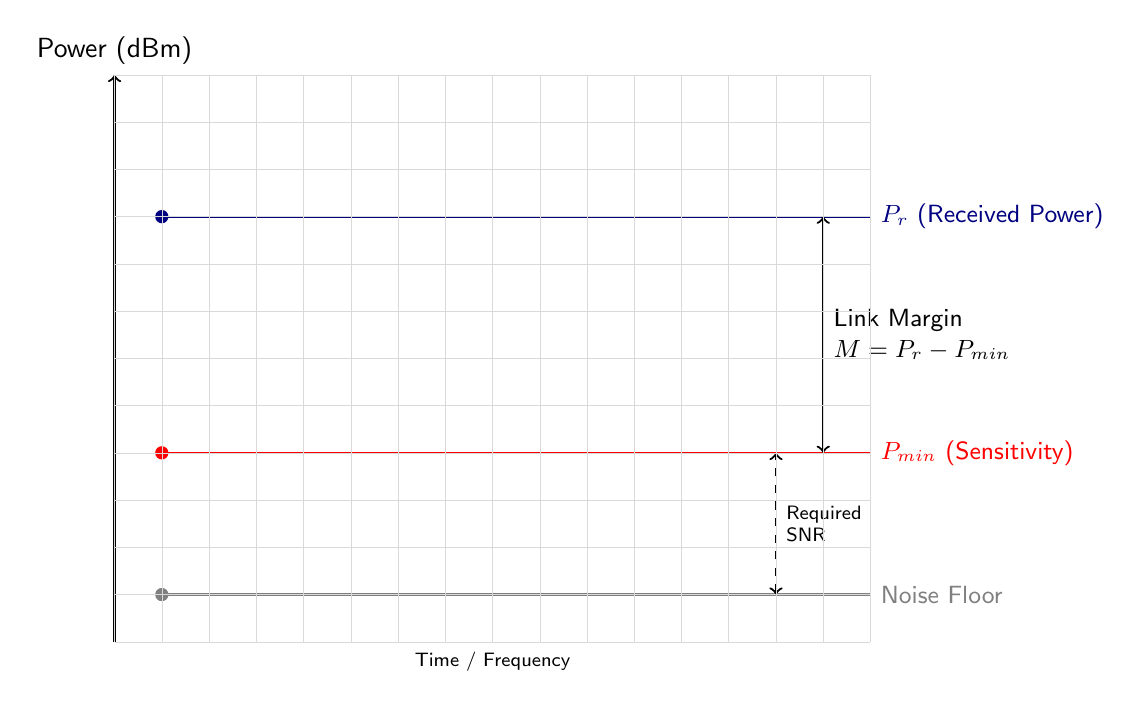
\begin{tikzpicture}[scale=1.2]
% Power levels
\draw[thick,->] (0,0) -- (0,6) node[above] {\sffamily Power (dBm)};

% Received power
\draw[thick, NavyBlue] (0.5,4.5) -- (8,4.5) node[right, font=\sffamily\small] {$P_r$ (Received Power)};
\fill[NavyBlue] (0.5,4.5) circle (2pt);

% Receiver sensitivity
\draw[thick, red] (0.5,2) -- (8,2) node[right, font=\sffamily\small] {$P_{\text{min}}$ (Sensitivity)};
\fill[red] (0.5,2) circle (2pt);

% Noise floor
\draw[thick, gray] (0.5,0.5) -- (8,0.5) node[right, font=\sffamily\small] {Noise Floor};
\fill[gray] (0.5,0.5) circle (2pt);

% Margin annotation
\draw[<->, thick] (7.5,2) -- (7.5,4.5) node[midway, right, align=left, font=\sffamily\small] {Link Margin\\$M = P_r - P_{\text{min}}$};

% Required SNR annotation
\draw[<->, thick, dashed] (7,0.5) -- (7,2) node[midway, right, align=left, font=\sffamily\scriptsize] {Required\\SNR};

% Grid
\draw[very thin, gray!30] (0,0) grid[step=0.5] (8,6);

% Labels
\node[below, font=\sffamily\scriptsize] at (4,0) {Time / Frequency};
\end{tikzpicture}
\end{center}

\section{Worked Example: WiFi Indoor Link}

\textbf{Scenario:} 2.4~GHz WiFi 802.11n link, 20~MHz channel, QPSK 1/2 coding, 50~m indoor range with wall penetration.

\subsection*{Given Parameters}

\begin{tabular}{@{}ll@{}}
Frequency & 2.4~GHz \\
Distance & 50~m \\
Modulation & QPSK, rate 1/2 \\
Bandwidth & 20~MHz \\
PA output & 20~dBm \\
TX cable loss & 0.5~dB \\
TX antenna gain & 2~dBi \\
Wall penetration & 2 walls $\times$ 5~dB $= 10$~dB \\
RX antenna gain & 0~dBi (laptop internal) \\
RX noise figure & 6~dB \\
Required SNR & 5~dB \\
Implementation loss & 2~dB \\
\end{tabular}

\subsection*{Step 1: Transmitter EIRP}

\begin{align}
P_t &= P_{\text{amp}} - L_{\text{TX}} = 20 - 0.5 = 19.5\text{~dBm} \notag \\
\text{EIRP} &= P_t + G_t = 19.5 + 2 = 21.5\text{~dBm}
\label{eq:ex1-eirp}
\end{align}

\subsection*{Step 2: Path Loss}

\begin{align}
L_{\text{FSPL}} &= 32.45 + 20\log_{10}(0.05) + 20\log_{10}(2400) \notag \\
&= 32.45 - 26 + 67.6 = 74.0\text{~dB} \notag \\
L_{\text{total}} &= L_{\text{FSPL}} + L_{\text{walls}} = 74 + 10 = 84\text{~dB}
\label{eq:ex1-path-loss}
\end{align}

\subsection*{Step 3: Received Power}

\begin{equation}
P_r = \text{EIRP} - L_{\text{total}} + G_r = 21.5 - 84 + 0 = -62.5\text{~dBm}
\label{eq:ex1-rx-power}
\end{equation}

\subsection*{Step 4: Receiver Sensitivity}

\begin{align}
N_0 &= -174\text{~dBm/Hz} + 10\log_{10}(20 \times 10^6) = -174 + 73 = -101\text{~dBm} \notag \\
P_{\text{min}} &= N_0 + \text{NF} + \text{SNR}_{\text{req}} + L_{\text{impl}} \notag \\
&= -101 + 6 + 5 + 2 = -88\text{~dBm}
\label{eq:ex1-sensitivity}
\end{align}

\subsection*{Step 5: Link Margin}

\begin{equation}
M = P_r - P_{\text{min}} = -62.5 - (-88) = 25.5\text{~dB}
\label{eq:ex1-margin}
\end{equation}

\begin{calloutbox}[colback=black!8!white,colframe=black]{Link Budget Summary}
\textbf{Result: Link closes with 25.5~dB margin}

This comfortable margin accommodates:
\begin{itemize}
\item Fast fading (Rayleigh/Rician)
\item Interference from adjacent networks
\item Component aging and temperature variations
\item Movement and multipath effects
\end{itemize}

\textbf{Conclusion:} Link is highly reliable for stationary indoor WiFi applications.
\end{calloutbox}

\section{Worked Example: GEO Satellite Ku-band Downlink}

\textbf{Scenario:} Geostationary satellite downlink at 12~GHz, 36,000~km slant range, 1~m receive dish, clear sky conditions.

\subsection*{Given Parameters}

\begin{tabular}{@{}ll@{}}
Frequency & 12~GHz (Ku-band) \\
Distance & 36,000~km (GEO orbit) \\
Satellite PA & 100~W $= 50$~dBm \\
TX antenna gain & 30~dBi (spot beam) \\
Atmospheric loss & 0.5~dB ($5°$ elevation) \\
Scintillation margin & 2~dB \\
RX dish diameter & 1~m \\
RX dish efficiency & 60\% \\
LNA noise figure & 0.8~dB (cryogenic) \\
Cable loss & 1~dB \\
Bandwidth & 36~MHz (DVB-S2) \\
Modulation & QPSK 3/4 with LDPC \\
Required SNR & 6.5~dB \\
Implementation loss & 1.5~dB \\
\end{tabular}

\subsection*{Step 1: Satellite EIRP}

\begin{equation}
\text{EIRP} = P_t + G_t = 50 + 30 = 80\text{~dBm}
\label{eq:ex2-eirp}
\end{equation}

\subsection*{Step 2: Path Loss}

\begin{align}
L_{\text{FSPL}} &= 32.45 + 20\log_{10}(36{,}000) + 20\log_{10}(12{,}000) \notag \\
&= 32.45 + 91.1 + 81.6 = 205.2\text{~dB} \notag \\
L_{\text{total}} &= L_{\text{FSPL}} + L_{\text{atm}} + L_{\text{scint}} \notag \\
&= 205.2 + 0.5 + 2.0 = 207.7\text{~dB}
\label{eq:ex2-path-loss}
\end{align}

\subsection*{Step 3: Receive Antenna Gain}

For a parabolic dish with diameter $D$ and efficiency $\eta$:
\begin{align}
G_r &= 10\log_{10}\left(\eta \left(\frac{\pi D}{\lambda}\right)^2\right) \notag \\
&= 10\log_{10}\left(0.6 \times \left(\frac{\pi \times 1}{0.025}\right)^2\right) \notag \\
&= 10\log_{10}(948) = 37.8\text{~dBi}
\label{eq:ex2-rx-gain}
\end{align}

\subsection*{Step 4: Received Power}

\begin{align}
P_r &= \text{EIRP} - L_{\text{total}} + G_r - L_{\text{cable}} \notag \\
&= 80 - 207.7 + 37.8 - 1 = -90.9\text{~dBm}
\label{eq:ex2-rx-power}
\end{align}

\subsection*{Step 5: Receiver Sensitivity}

\begin{align}
N_0 &= -174 + 10\log_{10}(36 \times 10^6) = -174 + 75.6 = -98.4\text{~dBm} \notag \\
P_{\text{min}} &= N_0 + \text{NF} + \text{SNR}_{\text{req}} + L_{\text{impl}} \notag \\
&= -98.4 + 0.8 + 6.5 + 1.5 = -89.6\text{~dBm}
\label{eq:ex2-sensitivity}
\end{align}

\subsection*{Step 6: Link Margin}

\begin{equation}
M = P_r - P_{\text{min}} = -90.9 - (-89.6) = -1.3\text{~dB}
\label{eq:ex2-margin}
\end{equation}

\begin{warningbox}
\textbf{Link fails!} Negative margin indicates the link cannot close under these conditions. The 1~m dish is insufficient.
\end{warningbox}

\subsection*{Solution: Increase Dish Size}

\textbf{Option 1: 1.8~m dish}
\begin{align*}
G_r &= 37.8 + 20\log_{10}(1.8) = 42.9\text{~dBi} \\
P_r &= 80 - 207.7 + 42.9 - 1 = -85.8\text{~dBm} \\
M &= -85.8 - (-89.6) = 3.8\text{~dB (marginal)}
\end{align*}

\textbf{Option 2: 2.4~m dish (recommended)}
\begin{align*}
G_r &= 37.8 + 20\log_{10}(2.4) = 45.4\text{~dBi} \\
P_r &= 80 - 207.7 + 45.4 - 1 = -83.3\text{~dBm} \\
M_{\text{clear}} &= -83.3 - (-89.6) = 6.3\text{~dB}
\end{align*}

With 5~dB rain margin for 99\% availability:
\begin{align*}
P_r(\text{rain}) &= -83.3 - 5 = -88.3\text{~dBm} \\
M_{\text{rain}} &= -88.3 - (-89.6) = 1.3\text{~dB (acceptable)}
\end{align*}

\begin{calloutbox}[colback=black!8!white,colframe=black]{Design Recommendation}
\textbf{Result: 2.4~m dish provides adequate margin}

\begin{itemize}
\item Clear-sky margin: 6.3~dB
\item Rain-faded margin: 1.3~dB (99\% availability)
\item Trades cost vs reliability
\end{itemize}

\textbf{Conclusion:} Link design requires careful margin analysis. Undersized antennas lead to outages; oversized antennas increase cost unnecessarily.
\end{calloutbox}

\section{Worked Example: Cellular LTE Link}

\textbf{Scenario:} LTE eNodeB (cell tower) to user equipment (UE) at 2.6~GHz, 10~MHz resource block, QPSK 1/2 coding, 5~km suburban environment with building penetration.

\subsection*{Given Parameters}

\begin{tabular}{@{}ll@{}}
Frequency & 2.6~GHz \\
Distance & 5~km \\
Modulation & QPSK, rate 1/2 Turbo \\
Bandwidth & 10~MHz \\
eNodeB PA & 43~dBm (20~W per antenna) \\
TX antenna gain & 17~dBi (sector antenna) \\
TX cable loss & 2~dB \\
Shadowing margin & 8~dB (90\% coverage) \\
Building penetration & 10~dB \\
UE antenna gain & $-2$~dBi (internal, near body) \\
UE noise figure & 9~dB \\
Required SNR & 4~dB \\
Implementation loss & 2~dB \\
\end{tabular}

\subsection*{Step 1: Transmitter EIRP}

\begin{equation}
\text{EIRP} = P_t + G_t - L_{\text{TX}} = 43 + 17 - 2 = 58\text{~dBm}
\label{eq:ex3-eirp}
\end{equation}

\subsection*{Step 2: Path Loss}

\begin{align}
L_{\text{FSPL}} &= 32.45 + 20\log_{10}(5) + 20\log_{10}(2600) \notag \\
&= 32.45 + 14.0 + 68.3 = 114.8\text{~dB} \notag \\
L_{\text{total}} &= L_{\text{FSPL}} + L_{\text{shadow}} + L_{\text{building}} \notag \\
&= 114.8 + 8 + 10 = 132.8\text{~dB}
\label{eq:ex3-path-loss}
\end{align}

\subsection*{Step 3: Received Power}

\begin{equation}
P_r = \text{EIRP} - L_{\text{total}} + G_r = 58 - 132.8 - 2 = -76.8\text{~dBm}
\label{eq:ex3-rx-power}
\end{equation}

\subsection*{Step 4: Receiver Sensitivity}

\begin{align}
N_0 &= -174 + 10\log_{10}(10 \times 10^6) = -174 + 70 = -104\text{~dBm} \notag \\
P_{\text{min}} &= N_0 + \text{NF} + \text{SNR}_{\text{req}} + L_{\text{impl}} \notag \\
&= -104 + 9 + 4 + 2 = -89\text{~dBm}
\label{eq:ex3-sensitivity}
\end{align}

\subsection*{Step 5: Link Margin}

\begin{equation}
M = P_r - P_{\text{min}} = -76.8 - (-89) = 12.2\text{~dB}
\label{eq:ex3-margin}
\end{equation}

\subsection*{Fading Considerations}

\textbf{Rayleigh fading (10~dB fade depth, 10\% of time):}
\begin{align*}
P_r(\text{fade}) &= -76.8 - 10 = -86.8\text{~dBm} \\
M(\text{fade}) &= -86.8 - (-89) = 2.2\text{~dB (marginal)}
\end{align*}

\textbf{With 2-antenna diversity (MRC):}
\begin{align*}
\text{Diversity gain} &= 5\text{~dB (typical for 2-branch)} \\
P_r(\text{fade+div}) &= -86.8 + 5 = -81.8\text{~dBm} \\
M(\text{fade+div}) &= -81.8 - (-89) = 7.2\text{~dB (improved)}
\end{align*}

\begin{calloutbox}[colback=black!8!white,colframe=black]{Mobile Link Analysis}
\textbf{Result: Link closes with 12.2~dB margin (static)}

Mobile considerations:
\begin{itemize}
\item Static/slow-moving UE: 12.2~dB margin (good)
\item Deep Rayleigh fade: 2.2~dB margin (service degradation)
\item With diversity: 7.2~dB margin in fade (acceptable)
\end{itemize}

\textbf{Conclusion:} Antenna diversity is critical for mobile cellular systems to maintain quality during fading. Single-antenna UE experiences intermittent outages in deep fades.
\end{calloutbox}

\section{Link Budget Table Template}

The following template provides a systematic framework for link budget calculations:

\begin{center}
\begin{tabular}{@{}p{0.25\linewidth}p{0.15\linewidth}p{0.12\linewidth}p{0.10\linewidth}p{0.28\linewidth}@{}}
\toprule
\textbf{Parameter} & \textbf{Symbol} & \textbf{Value} & \textbf{Units} & \textbf{Notes} \\
\midrule
\multicolumn{5}{l}{\textbf{TRANSMITTER}} \\
TX power (PA) & $P_{\text{amp}}$ & --- & dBm & \\
TX losses & $L_{\text{TX}}$ & --- & dB & Cables, filters \\
Transmit power & $P_t$ & --- & dBm & $P_{\text{amp}} - L_{\text{TX}}$ \\
TX antenna gain & $G_t$ & --- & dBi & \\
\textbf{EIRP} & --- & --- & dBm & $P_t + G_t$ \\
\midrule
\multicolumn{5}{l}{\textbf{PROPAGATION}} \\
Distance & $d$ & --- & km & \\
Frequency & $f$ & --- & GHz & \\
Free-space loss & $L_{\text{FSPL}}$ & --- & dB & Eq.~\ref{eq:fspl-practical} \\
Atmospheric loss & $L_{\text{atm}}$ & --- & dB & \\
Rain attenuation & $L_{\text{rain}}$ & --- & dB & ITU-R model \\
Other losses & $L_{\text{other}}$ & --- & dB & Multipath, etc. \\
\textbf{Total path loss} & $L_{\text{total}}$ & --- & dB & Sum of above \\
\midrule
\multicolumn{5}{l}{\textbf{RECEIVER}} \\
RX antenna gain & $G_r$ & --- & dBi & \\
RX losses & $L_{\text{RX}}$ & --- & dB & Cables, connectors \\
\textbf{Received power} & $P_r$ & --- & dBm & Eq.~\ref{eq:link-budget-complete} \\
\midrule
\multicolumn{5}{l}{\textbf{PERFORMANCE}} \\
Bandwidth & $B$ & --- & MHz & \\
Thermal noise & $N_0$ & $-174 + 10\log(B)$ & dBm & \\
Noise figure & NF & --- & dB & \\
Required SNR & $\text{SNR}_{\text{req}}$ & --- & dB & For target BER \\
Impl. loss & $L_{\text{impl}}$ & --- & dB & Typically 1--3~dB \\
\textbf{Sensitivity} & $P_{\text{min}}$ & --- & dBm & Eq.~\ref{eq:receiver-sensitivity} \\
\midrule
\textbf{MARGIN} & $M$ & --- & dB & $P_r - P_{\text{min}}$ \\
\bottomrule
\end{tabular}
\end{center}

\section{Fade Margin Design Guidelines}

System designers must allocate sufficient margin to accommodate various impairments. The total margin requirement depends on the propagation environment and target availability.

\subsection{Clear-Sky Margin}

Minimum margin required under ideal propagation conditions:

\begin{itemize}
\item \textbf{Satellite (GEO Ku/Ka-band):} 5--10~dB
\item \textbf{Terrestrial line-of-sight:} 10--15~dB
\item \textbf{Mobile non-line-of-sight:} 15--20~dB
\end{itemize}

\subsection{Rain Margin (Satellite)}

Additional margin for rain attenuation depends on target availability:

\begin{center}
\begin{tabular}{@{}lll@{}}
\toprule
\textbf{Availability} & \textbf{Ku-band} & \textbf{Ka-band} \\
\midrule
99.0\% & 5--8~dB & 10--15~dB \\
99.9\% & 10--15~dB & 20--25~dB \\
99.99\% & 20--30~dB & 30--40~dB \\
\bottomrule
\end{tabular}
\end{center}

\subsection{Multipath Fading Margin}

For mobile and urban environments:

\begin{itemize}
\item \textbf{Rayleigh fading:} 20--30~dB for 90\% location reliability
\item \textbf{Rician fading ($K = 6$~dB):} 10--15~dB
\end{itemize}

\subsection{Total Margin Budget}

\begin{equation}
M_{\text{total}} = M_{\text{clear}} + M_{\text{rain}} + M_{\text{fade}}
\label{eq:total-margin}
\end{equation}

Figure~\ref{fig:fade-margin} illustrates the margin allocation strategy.

\begin{center}
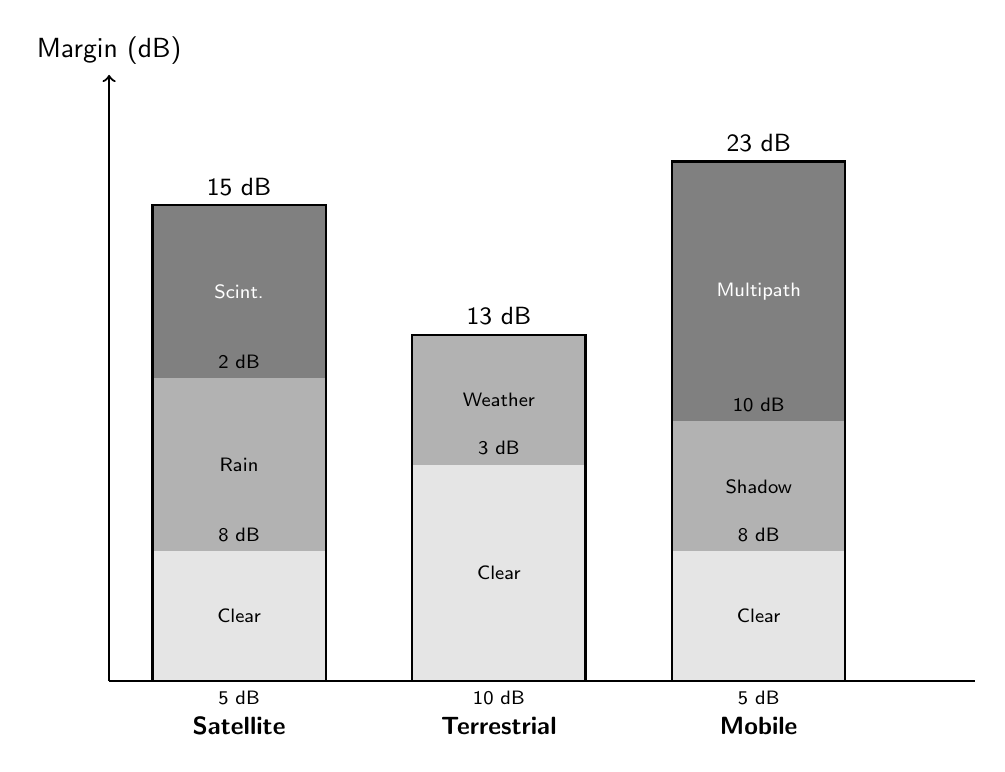
\begin{tikzpicture}[scale=1.1]
% Stacked bar chart showing margin allocation
\draw[thick,->] (0,0) -- (0,7) node[above] {\sffamily Margin (dB)};
\draw[thick] (0,0) -- (10,0);

% Satellite example
\fill[black!10] (0.5,0) rectangle (2.5,1.5);
\node[font=\sffamily\scriptsize] at (1.5,0.75) {Clear};
\node[below, font=\sffamily\scriptsize] at (1.5,0) {5 dB};

\fill[black!30] (0.5,1.5) rectangle (2.5,3.5);
\node[font=\sffamily\scriptsize] at (1.5,2.5) {Rain};
\node[above, font=\sffamily\scriptsize] at (1.5,1.5) {8 dB};

\fill[black!50] (0.5,3.5) rectangle (2.5,5.5);
\node[font=\sffamily\scriptsize, text=white] at (1.5,4.5) {Scint.};
\node[above, font=\sffamily\scriptsize] at (1.5,3.5) {2 dB};

\draw[thick] (0.5,0) rectangle (2.5,5.5);
\node[below, font=\sffamily\small\bfseries] at (1.5,-0.3) {Satellite};
\node[above, font=\sffamily\small] at (1.5,5.5) {15 dB};

% Terrestrial LOS
\fill[black!10] (3.5,0) rectangle (5.5,2.5);
\node[font=\sffamily\scriptsize] at (4.5,1.25) {Clear};
\node[below, font=\sffamily\scriptsize] at (4.5,0) {10 dB};

\fill[black!30] (3.5,2.5) rectangle (5.5,4);
\node[font=\sffamily\scriptsize] at (4.5,3.25) {Weather};
\node[above, font=\sffamily\scriptsize] at (4.5,2.5) {3 dB};

\draw[thick] (3.5,0) rectangle (5.5,4);
\node[below, font=\sffamily\small\bfseries] at (4.5,-0.3) {Terrestrial};
\node[above, font=\sffamily\small] at (4.5,4) {13 dB};

% Mobile NLOS
\fill[black!10] (6.5,0) rectangle (8.5,1.5);
\node[font=\sffamily\scriptsize] at (7.5,0.75) {Clear};
\node[below, font=\sffamily\scriptsize] at (7.5,0) {5 dB};

\fill[black!30] (6.5,1.5) rectangle (8.5,3);
\node[font=\sffamily\scriptsize] at (7.5,2.25) {Shadow};
\node[above, font=\sffamily\scriptsize] at (7.5,1.5) {8 dB};

\fill[black!50] (6.5,3) rectangle (8.5,6);
\node[font=\sffamily\scriptsize, text=white] at (7.5,4.5) {Multipath};
\node[above, font=\sffamily\scriptsize] at (7.5,3) {10 dB};

\draw[thick] (6.5,0) rectangle (8.5,6);
\node[below, font=\sffamily\small\bfseries] at (7.5,-0.3) {Mobile};
\node[above, font=\sffamily\small] at (7.5,6) {23 dB};

\end{tikzpicture}
\end{center}

\begin{keyconcept}
\textbf{Trade-off:} Higher margin increases link reliability but requires larger antennas, more transmit power, or lower data rates. Cost-optimized designs balance margin against system requirements.
\end{keyconcept}

\section{Adaptive Techniques}

\subsection{Adaptive Coding and Modulation (ACM)}

ACM dynamically adjusts modulation order and coding rate based on instantaneous channel conditions, maximizing spectral efficiency while maintaining connectivity.

\textbf{Principle:} Select modulation/coding combination that maximizes throughput for current SNR.

\begin{calloutbox}{Example: DVB-S2X Satellite ACM}
\textbf{Operating modes:}

\begin{center}
\begin{tabular}{@{}llll@{}}
\toprule
\textbf{Conditions} & \textbf{ModCod} & \textbf{Spectral Eff.} & \textbf{Required C/N} \\
\midrule
Clear sky & 32APSK 9/10 & 3.5~bps/Hz & 16~dB \\
Light rain & 8PSK 3/4 & 2.25~bps/Hz & 11~dB \\
Heavy rain & QPSK 1/2 & 1.0~bps/Hz & 4~dB \\
\bottomrule
\end{tabular}
\end{center}

\textbf{Benefit:} Throughput adapts gracefully to channel degradation. Link maintains connectivity even during severe fades at reduced data rate.
\end{calloutbox}

\subsection{Link Availability}

Link availability quantifies the percentage of time the link meets performance requirements:
\begin{equation}
\text{Availability} = \frac{\text{Time link operational}}{\text{Total time}} \times 100\%
\label{eq:availability}
\end{equation}

\textbf{Target availability by application:}

\begin{center}
\begin{tabular}{@{}lll@{}}
\toprule
\textbf{Application} & \textbf{Availability} & \textbf{Downtime/year} \\
\midrule
Data networks & 99.9\% & 8.76~hours \\
Voice telephony & 99.99\% & 52.6~minutes \\
Mission-critical & 99.999\% & 5.26~minutes \\
\bottomrule
\end{tabular}
\end{center}

\subsection{Rain Statistics and Design}

For satellite Ku/Ka-band links, rain is the dominant availability-limiting factor.

\textbf{ITU rain statistics:}
\begin{itemize}
\item \textbf{Temperate climate:} 12~mm/hr exceeded 1\% of time (3.65~days/year)
\item \textbf{Tropical climate:} 42~mm/hr exceeded 1\% of time
\end{itemize}

\textbf{Design procedure:}
\begin{enumerate}
\item Choose target availability (e.g., 99.9\%)
\item Determine rain rate exceeded $(100 - 99.9) = 0.1\%$ of time
\item Calculate rain attenuation using ITU-R model (Eq.~\ref{eq:rain-attenuation})
\item Ensure clear-sky margin $\geq$ rain attenuation
\end{enumerate}

\section{Applications}

Link budget analysis is fundamental to the design and operation of wireless communication systems across diverse applications:

\subsection{Satellite Communications}

\begin{itemize}
\item \textbf{GEO broadcast (TV, radio):} Massive path loss (200+~dB) requires high EIRP, large ground station antennas
\item \textbf{LEO constellations (Starlink, OneWeb):} Lower path loss but rapid satellite motion requires beam steering
\item \textbf{Deep-space missions (Voyager, Mars rovers):} Extreme distances demand every millidecibel of margin
\end{itemize}

\subsection{Cellular Networks}

\begin{itemize}
\item \textbf{Coverage planning:} Cell tower placement based on link budget to achieve target coverage area
\item \textbf{Capacity optimization:} Balance transmit power, antenna height, frequency reuse
\item \textbf{5G mmWave:} High path loss and rain attenuation require dense small-cell deployment
\end{itemize}

\subsection{WiFi and Wireless LANs}

\begin{itemize}
\item \textbf{Access point placement:} Indoor propagation dominated by wall/floor penetration losses
\item \textbf{Range extension:} External antennas, higher transmit power, or mesh networks
\item \textbf{Interference management:} Margin allocation for co-channel and adjacent-channel interference
\end{itemize}

\subsection{Point-to-Point Microwave}

\begin{itemize}
\item \textbf{Backhaul links:} Fiber alternative for cellular/internet infrastructure
\item \textbf{High availability required:} 99.999\% typical, requires substantial rain margin
\item \textbf{Frequency selection:} Higher frequencies offer more bandwidth but suffer greater rain attenuation
\end{itemize}

\subsection{Radar and Sensing}

\begin{itemize}
\item \textbf{Weather radar:} Two-way link budget accounts for round-trip path loss
\item \textbf{Automotive radar (77~GHz):} Short range but high attenuation in rain/fog
\item \textbf{Synthetic aperture radar (SAR):} Extreme sensitivity requirements for earth observation
\end{itemize}

\section{Summary}

\textbf{Link budget essentials:}

\begin{enumerate}
\item \textbf{EIRP} $=$ TX power $+$ TX antenna gain (dBm)
\item \textbf{Path loss} $=$ FSPL $+$ atmospheric $+$ rain $+$ other (dB)
\item \textbf{Received power} $=$ EIRP $-$ path loss $+$ RX gain $-$ RX losses (dBm)
\item \textbf{Sensitivity} $=$ Noise floor $+$ NF $+$ SNR$_{\text{req}}$ $+$ implementation loss (dBm)
\item \textbf{Margin} $=$ Received power $-$ sensitivity (dB, \textbf{must be positive})
\end{enumerate}

\textbf{Design targets:}
\begin{itemize}
\item Clear-sky margin: $10+$~dB
\item Rain margin (satellite): 5--20~dB (depends on frequency, availability)
\item Total margin: 15--30~dB typical
\end{itemize}

\begin{keyconcept}
\textbf{Link budget is systematic accounting of all gains/losses from transmitter to receiver.} Start with EIRP, subtract path losses, add receiver gain, compare to sensitivity. Positive margin ensures link closure. Design for adequate margin (10--30~dB) to handle fading, rain, interference, and aging. Adaptive techniques (ACM, diversity) maximize throughput while maintaining connectivity.
\end{keyconcept}

\section{Further Reading}

\begin{itemize}
\item \textbf{Chapter~\ref{ch:fspl}:} Free-Space Path Loss---dominant loss mechanism in link budget
\item \textbf{Chapter~\ref{ch:snr}:} Signal-to-Noise Ratio---determines required carrier-to-noise ratio
\item \textbf{Chapter~\ref{ch:noise-figure}:} Noise Sources \& Noise Figure---receiver sensitivity calculation
\item \textbf{Chapter~\ref{ch:eb-n0}:} Energy Ratios ($E_s/N_0$ and $E_b/N_0$)---alternative SNR metrics
\item \textbf{Chapter~\ref{ch:rain-fade}:} Weather Effects---rain fade and fog attenuation for margin design
\item \textbf{Chapter~\ref{ch:multipath}:} Multipath Propagation \& Fading---Rayleigh and Rician fading for mobile links
\item \textbf{Chapter~\ref{ch:ber}:} Bit Error Rate---performance metric versus SNR
\item \textbf{Chapter~\ref{ch:modulation}:} Digital Modulation---impact on required SNR and spectral efficiency
\item \textbf{Chapter~\ref{ch:fec}:} Forward Error Correction---coding gain reduces required margin
\item \textbf{Chapter~\ref{ch:diversity}:} Antenna Diversity---improves margin in fading channels
\end{itemize}
